\documentclass{article}
\usepackage{fancyhdr}
\usepackage{extramarks}
\usepackage{amsmath}
\usepackage{amsthm}
\usepackage{amsfonts}
\usepackage{tikz}
\usepackage[plain]{algorithm}
\usepackage{algpseudocode}
\usepackage{listings} 
\usepackage{amssymb}
\usetikzlibrary{automata,positioning}

\usepackage{color}

\definecolor{dkgreen}{rgb}{0,0.6,0}
\definecolor{gray}{rgb}{0.5,0.5,0.5}
\definecolor{mauve}{rgb}{0.58,0,0.82}

\lstset{frame=tb,
  language=Python,
  aboveskip=3mm,
  belowskip=3mm,
  showstringspaces=false,
  columns=flexible,
  basicstyle={\small\ttfamily},
  numbers=none,
  numberstyle=\tiny\color{gray},
  keywordstyle=\color{blue},
  commentstyle=\color{dkgreen},
  stringstyle=\color{mauve},
  breaklines=true,
  breakatwhitespace=true,
  tabsize=3
}
%
% Basic Document Settings
%

\topmargin=-0.45in
\evensidemargin=0in
\oddsidemargin=0in
\textwidth=6.5in
\textheight=9.0in
\headsep=0.25in

\linespread{1.1}

\pagestyle{fancy}
\lhead{\hmwkAuthorName}
\chead{\hmwkClass\: \hmwkTitle}
\rhead{\firstxmark}
\lfoot{\lastxmark}
\cfoot{\thepage}

\renewcommand\headrulewidth{0.4pt}
\renewcommand\footrulewidth{0.4pt}

\setlength\parindent{0pt}

%
% Create Problem Sections
%

\newcommand{\enterProblemHeader}[1]{
    \nobreak\extramarks{}{Problem \arabic{#1} continued on next page\ldots}\nobreak{}
    \nobreak\extramarks{Problem \arabic{#1} (continued)}{Problem \arabic{#1} continued on next page\ldots}\nobreak{}
}

\newcommand{\exitProblemHeader}[1]{
    \nobreak\extramarks{Problem \arabic{#1} (continued)}{Problem \arabic{#1} continued on next page\ldots}\nobreak{}
    \stepcounter{#1}
    \nobreak\extramarks{Problem \arabic{#1}}{}\nobreak{}
}

\setcounter{secnumdepth}{0}
\newcounter{partCounter}
\newcounter{homeworkProblemCounter}
\setcounter{homeworkProblemCounter}{1}
\nobreak\extramarks{Problem \arabic{homeworkProblemCounter}}{}\nobreak{}

%
% Homework Problem Environment
%
% This environment takes an optional argument. When given, it will adjust the
% problem counter. This is useful for when the problems given for your
% assignment aren't sequential. See the last 3 problems of this template for an
% example.
%
\newenvironment{homeworkProblem}[1][-1]{
    \ifnum#1>0
        \setcounter{homeworkProblemCounter}{#1}
    \fi
    \section{Problem \arabic{homeworkProblemCounter}}
    \setcounter{partCounter}{1}
    \enterProblemHeader{homeworkProblemCounter}
}{
    \exitProblemHeader{homeworkProblemCounter}
}

%
% Homework Details
%   - Title
%   - Due date
%   - Class
%   - Section/Time
%   - Instructor
%   - Author
%
\newcommand{\hmwkNum}{6}
\newcommand{\hmwkTitle}{Homework\ \#\hmwkNum}
\newcommand{\hmwkDueDate}{October 31, 2019}
\newcommand{\hmwkClass}{CSCI971 Advance Computer Security}
\newcommand{\hmwkClassInstructor}{Chen Jiageng}
\newcommand{\hmwkAuthorName}{\textbf{Mei Wangzhihui}}
\newcommand{\hmwkAuthorNum}{\textbf{2019124044}}
%
% Title Page
%

\title{
    \vspace{2in}
    \textmd{\textbf{\hmwkClass:\\ \hmwkTitle}}\\
    % \normalsize\vspace{0.1in}\small{Due\ on\ \hmwkDueDate\ at 3:10pm}\\
    % \vspace{0.1in}\large{\textit{\hmwkClassInstructor\ \hmwkClassTime}}
    \vspace{3in}
}

\author{\hmwkAuthorName\ \\ \hmwkAuthorNum}
\date{}

\renewcommand{\part}[1]{\textbf{\large Part \Alph{partCounter}}\stepcounter{partCounter}\\}

%
% Various Helper Commands
%

% Useful for algorithms
\newcommand{\alg}[1]{\textsc{\bfseries \footnotesize #1}}

% For derivatives
\newcommand{\deriv}[1]{\frac{\mathrm{d}}{\mathrm{d}x} (#1)}

% For partial derivatives
\newcommand{\pderiv}[2]{\frac{\partial}{\partial #1} (#2)}

% Integral dx
\newcommand{\dx}{\mathrm{d}x}

% Alias for the Solution section header
\newcommand{\solution}{\textbf{\large Solution}}

% Probability commands: Expectation, Variance, Covariance, Bias
\newcommand{\E}{\mathrm{E}}
\newcommand{\Var}{\mathrm{Var}}
\newcommand{\Cov}{\mathrm{Cov}}
\newcommand{\Bias}{\mathrm{Bias}}

\begin{document}

\maketitle

\pagebreak

\begin{homeworkProblem}
\textbf{Solution:} \\
\textbf{a)\ How does a Merkle tree work?}\\
The original message are a sequence of l-bit blocks $x_1,x_2,...,x_n$. We just verify several blocks which are used in in the block set to minimize the computation size. Each block can be verified independently.

The Merkle tree applied collision resistant function $h$ to each block in $(x_1,x_2,...,x_n)\in \mathcal{X}^n$ get the accordant hash value set $(y_1,y_2,...,y_n)\in \mathcal{Y}^n$ by the algorithm:\\
for i = 1 to n, $y_i\leftarrow h(x_i)$

Then applied $h$ to $(y_1,y_2,...,y_n)$ to get the parental nodes $(y_{n+1},..., y_{2n+1})$ by the algorithm:

for i = 1 to n-1 , $y_{i+n}\leftarrow h(y_{2i-1},y_{2i})$\\
So we get an binary tree with $2n+1$ nodes.

When we want to verify the ith block ($\hat{x_i}=x_i?$), the algorithm need \textbf{Merkle proof} $\pi$, which is the intermediate hashes  of siblings of nodes on the path from i to root. For example, set $i=5, n=8$, then $\pi=(y_6,y_{12},y_{13})$. 

We then do hash computation for $\hat{x_i}$ from ith node position to root. In this example, calculate:\\
$\hat{y_5} \leftarrow h(\hat{x_5})\\ \hat{y_{11}}=h(\hat{y_5},y_6)\\\hat{y_{15}}=h(\hat{y_{11}}, y_{13})$

If $\hat{y_{15}}=y_{15}$, then $hat{x_5}$ is verified, else not. 
\\

\textbf{b)\ Why is it efficient when using Merkle tree to prove membership?}\\
As the computation complexity for binary tree from leaf to root is $O(log_2^n)$, so the there need $log_2^n$ times of hash computation in the verification process. 

Also, Merkle tree algorithm need not secret keys.
\\

\textbf{c)\ How to take advantage of a Merkle tree to prove non-membership?}\\
Suppose verifier want to verify that $x$ is not in the list $T$, The verifier sort all the elements in $T$, and then build Merkle tree, this is sorted Merkle tree. 

The verifier then find two adjancent leaves $x_{i},x_{i+1}$ and it satify that $x_{i}<x<x_{i+1}$. Next, verifier check Merkle proofs of $x_{i},x_{i+1}$, to make sure $x_{i},x_{i+1}$ is in the Merkle tree. If $x\neq x_{i}$ and $x\neq x_{i+1}$ then $x$ is not int the $T$, as $x_{i}$ and $x_{i+1}$ are adjancent leaf nodes. Else, $x$ may be either $x_{i}$ or $x_{i+1}$, so $x$ is in the $T$. 
\\

\textbf{d)\ How does blockchain use Merkle tree to verify transactions? Please describe by concrete example.}\\
\begin{figure}
    \centering %图片居中
    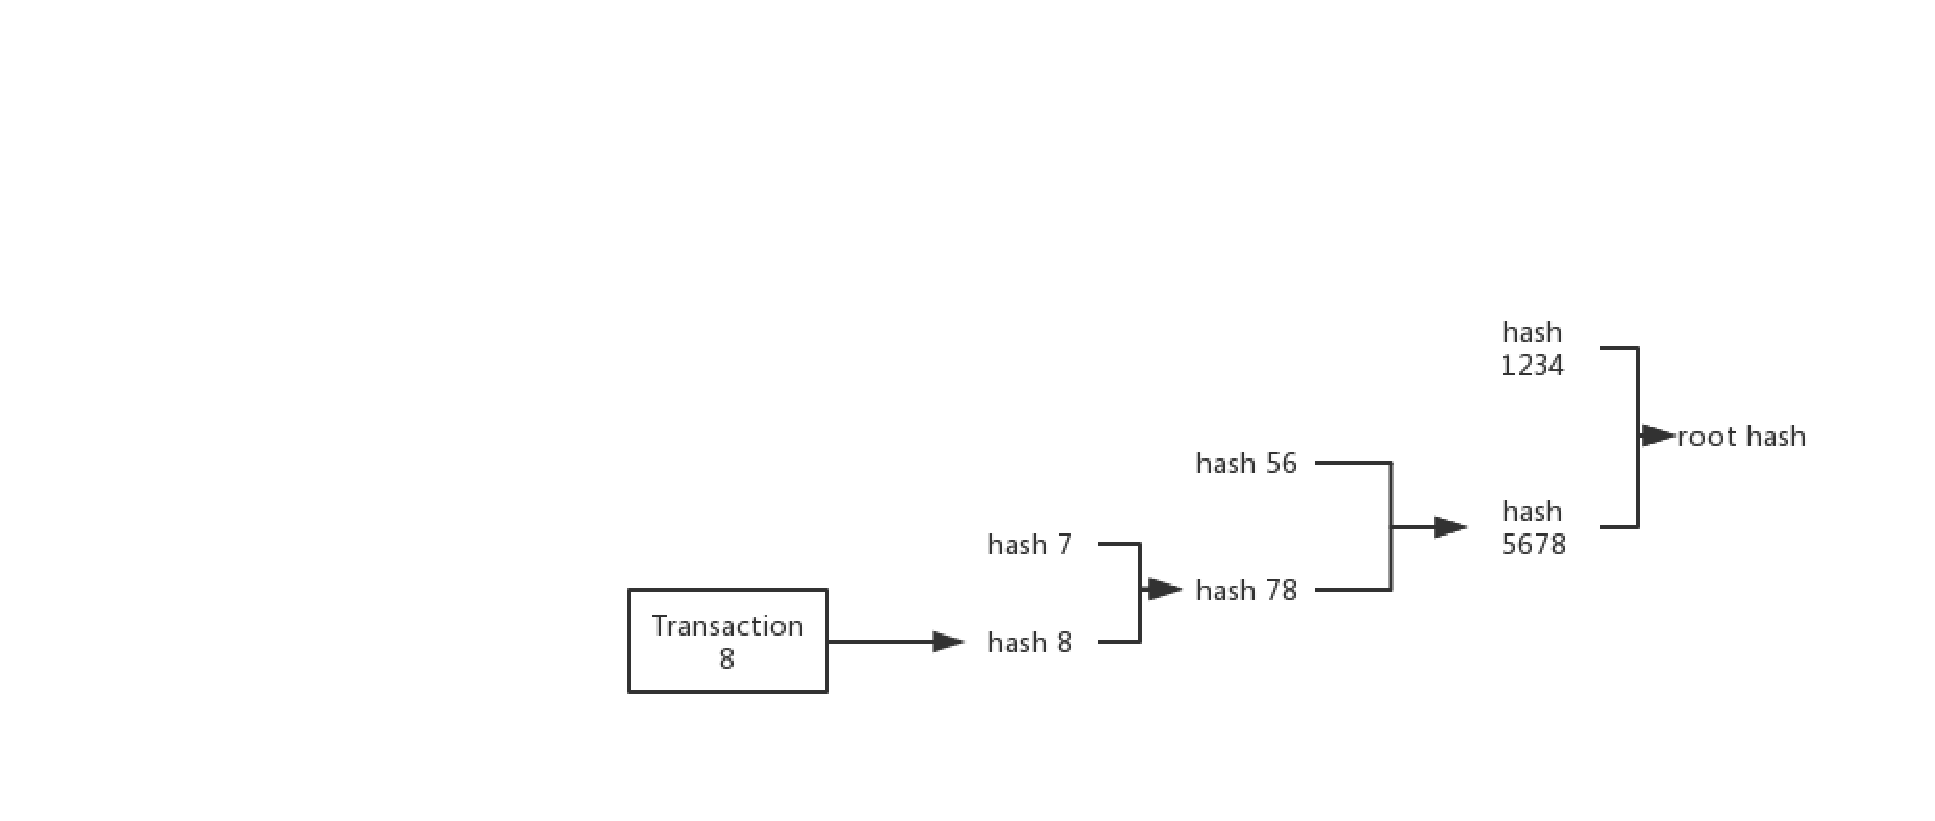
\includegraphics[width=1.0\textwidth]{blockchain} %插入图片,[]中设置图片大小,{}中是图片文件名
    \caption{Blockchain transaction verification in Merkle tree} %最终文档中希望显示的图片标题
    \label{blockchain} %用于文内引用的标签
\end{figure}


In the blockchain, each transaction need to be verified. The Merkle root maintain the integrity of all transaction data, which is stored in the block header. Each leaf node is hash of transactional data and non-leaf node is a hash of its previous hashes. As Merkle tree arebinary so it require even number of leaf nodes. If the number of nodes is odd, the last hash will be duplicated once to create an even number of leaf nodes.

We assume that transaction 8 happened in Figure \ref{blockchain} need verification. So verifier need not download the whole data but just the siblings hash nodes from its hash leaf to root, that is hash7, hash56, hash 1234, root hash. Apply hash computation with hash8 by the order, and the the transaction can be verified. The computation complexity is $O(log_2^n)$.


\end{homeworkProblem}
\end{document}


